\documentclass[12pt]{article}
\usepackage{graphicx}
\usepackage{parskip}
\usepackage{caption}
\usepackage{subcaption}
% test by saloni
% The following parameters seem to provide a reasonable page setup.
\topmargin 0.0cm
\oddsidemargin 0.2cm
\textwidth 17cm 
\textheight 21cm
\footskip 1.0cm


%The next command sets up an environment for the abstract to your paper.
\newenvironment{sciabstract}{%
\begin{quote} \bf}
{\end{quote}}

\newcounter{lastnote}
\newenvironment{scilastnote}{%
\setcounter{lastnote}{\value{enumiv}}%
\addtocounter{lastnote}{+1}%
\begin{list}%
{\arabic{lastnote}.}
{\setlength{\leftmargin}{.22in}}
{\setlength{\labelsep}{.5em}}}
{\end{list}}



\title{\vspace{-4cm}\textit{CS7038 Group B}\hspace{0.75cm}\\\line(1, 0){350}
} 
\author
{\vspace{-1.2cm}\\Hao Guan, Yaffy Koyo, Saloni Sharma \& Jeremiah Dunn\\\line(1, 0){350}}
\date{}

\begin{document} 

\maketitle 

\section{Theme}

In our game the player controls a maintenance robot on board a spaceship on a long journey. While on the journey the ship malfunctions and begins shutting down, the whole crew are in stasis and it is up to the robot to restore power.

The player must traverse the ship, reactivating components and lighting the ship up in the process. The gameplay takes inspiration from exploration based platformer games such as \textit{Spelunker}.

\section{Gameplay}




Movement and jumping will be implemented using Unity's 2D physics engine to handle.

Re-activating components of the ship has a probability of activating some of the ship's security measures. These will include activating traps or spawning hostile defence drones. On reaching the next component these security systems can be deactivated.

\begin{figure}[ht]
\centering
\begin{subfigure}{.5\textwidth}
  \centering
  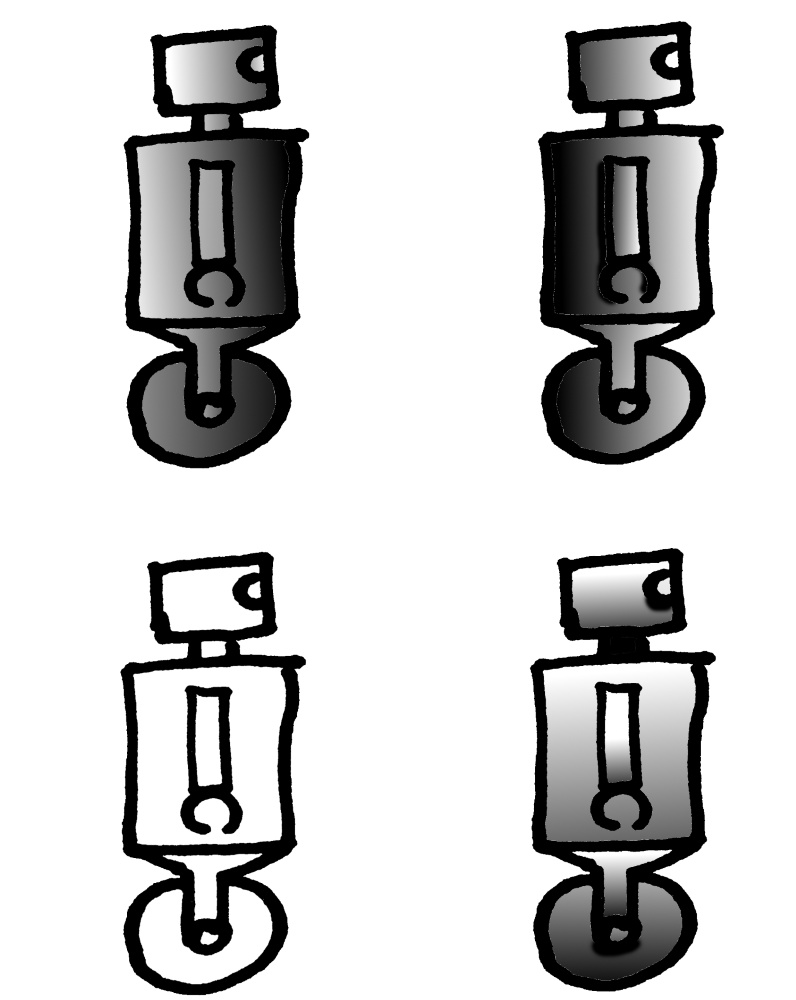
\includegraphics[scale=0.2, trim = 0cm 0cm 0cm 2cm]{images/in}
  \caption{input files including a base file and the same file drawn as if it was lit from a handful of different directions}
  \label{fig:sub1:pl}
\end{subfigure}%
\begin{subfigure}{.5\textwidth}
  \centering
  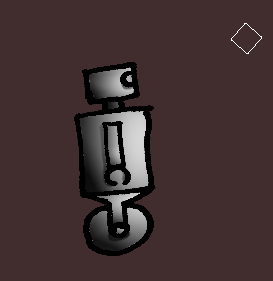
\includegraphics[scale=0.9, trim = 0cm 0cm 0cm 0.5cm]{images/out}	
  \caption{output file reacting to a dynamic light shown by the white cube}
  \label{fig:sub2:pl}
\end{subfigure}
\caption{Player character mock-up}
\label{fig:player}
\end{figure}

We plan to use 2d sprites, with normal maps created using \textit{SpriteLamp} for the game's lighting effects. Figure~\ref{fig:player} shows an example of it's use.


\section{Level Generation}

The game will use elements of procedural generation to create levels. To do this, first a grid of \textit{rooms} is created as shown in figure~\ref{fig:sub1:level}. A random position on the top of the grid is chosen to be the starting room. From here there is a probability of stepping left/right or down. If the stepping algorithm reaches a wall it will automatically step down. At the bottom of the grid the probability of stepping down is replaced with the probability of creating a level end.

\begin{figure}[ht]
\centering
\begin{subfigure}{.5\textwidth}
  \centering
  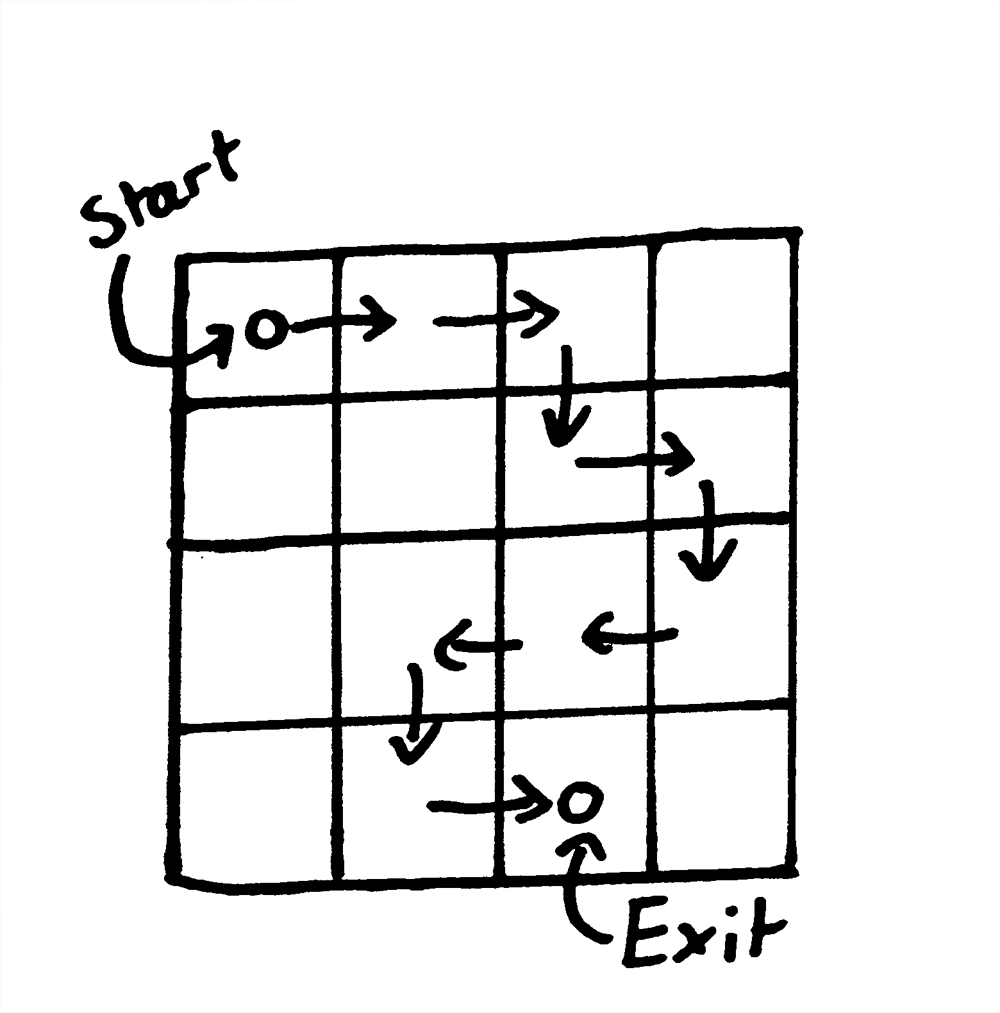
\includegraphics[scale=0.2, trim = 0cm 0cm 0cm 2cm]{images/4x4}
  \caption{Room grid}
  \label{fig:sub1:level}
\end{subfigure}%
\begin{subfigure}{.5\textwidth}
  \centering
  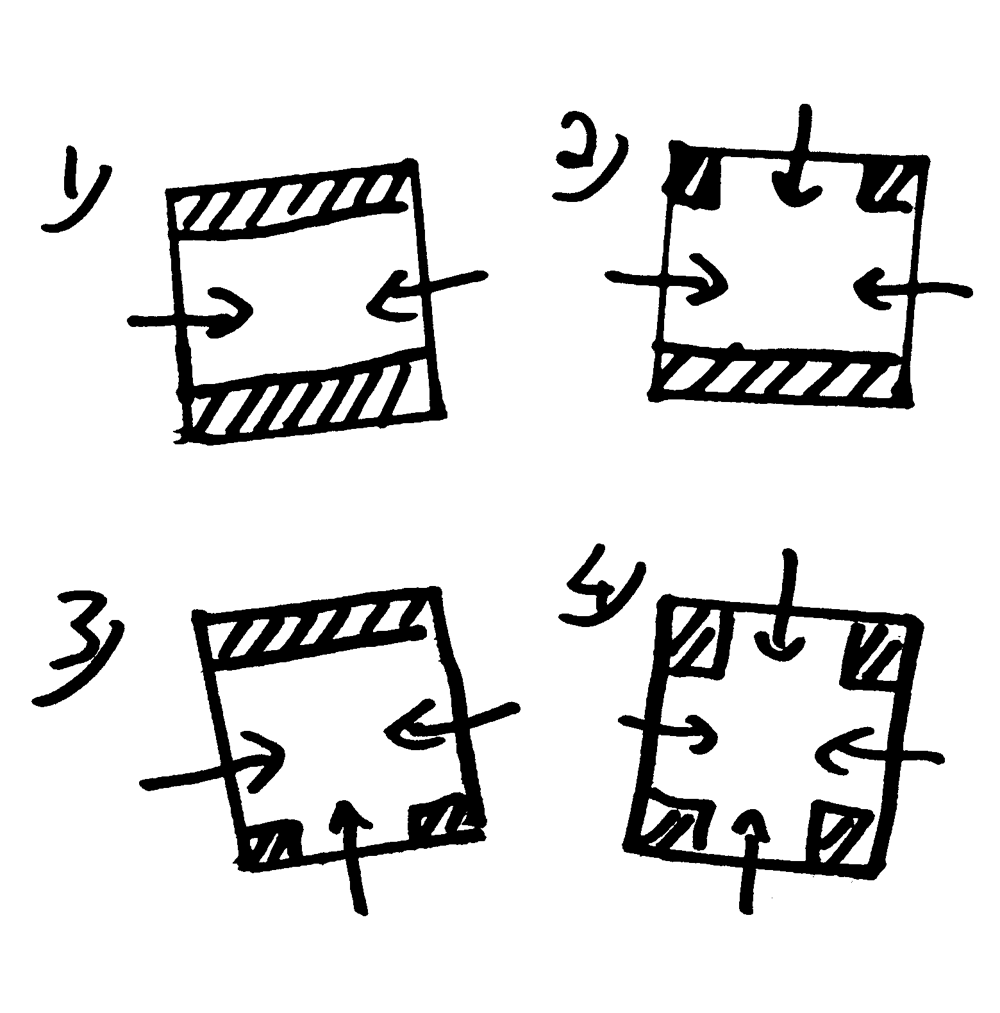
\includegraphics[scale=0.2, trim = 0cm 0cm 0cm 2cm]{images/16x16}	
  \caption{Different rooms, hashed areas represent floor/roof}
  \label{fig:sub2:level}
\end{subfigure}
\caption{Level Generation}
\label{fig:level_gen}
\end{figure}


After the room grid is created the individual rooms are populated with pre-existing room tiles. To get a basic version of the game running only the four room tiles show in figure~\ref{fig:sub2:level} would be needed with solid rooms for the rooms off the solution path. Individual rooms will be tile based and will be stored in text files which the game will read in and then populate.


\section{Management \& Version Control Software}
For version control we are using git. To manage creating stories, logging time and creating burn down charts we are using JIRA which is deployed on one of our machines.
\section{Project management}
After a week of discussion on the game project idea, all main tasks were subdivided into Epics: \textit{level generation, GUI, game logic} and the \textit{character controller}. 

The epics are spread over the duration of the project and are broken down into a number of smaller stories as shown in figure~\ref{fig:backlog}. Tasks for each sprints will be chosen from the backlog based on their priority and requirements.

The project will be divided into 4 sprints. At the start of each week we will have a grooming and kick-off meeting. In the grooming meeting we will look through the backlog and see what stories we want to work on, assign story points and flesh out the descriptions or subtask them as required. In the kick-off we will assign tasks and give time estimates.

\begin{figure}[ht]
\centering
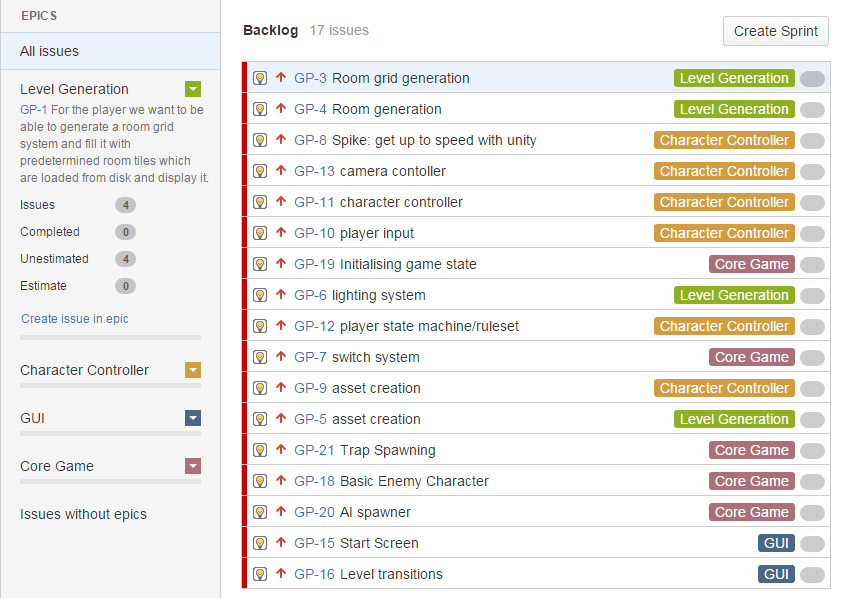
\includegraphics[scale = 0.8]{images/backlog.png}
\caption{Screenshot of Storyboard on Jira}
\label{fig:backlog}
\end{figure}
\section{Meeting Plan}
Sprint-Plan meetings would organized in the beginning of each sprint to discuss about the execution plan for the sprint tasks and Sprint-Demo meetings would be organised to discuss and demonstrate the executed sprint tasks.

The team will have stand-ups or kick-off/grooming meetings three times a week. Stand ups will aim to last for 10 minutes with any additional discussions happening in separate meetings outside this time.



%%%%%%%%%%%%%%%%%%%%%%%
% sample figure code
%%%%%%%%%%%%%%%%%%%%%%%
%\begin{figure}
%\centering
%\includegraphics[scale=0.4, trim = 0cm 0cm 0cm 0cm]{images/test}
%\label{fig:some_label}
%\caption{some figure}
%\end{figure}




\end{document}




















